% !Mode:: "TeX:UTF-8"
% !TEX program  = xelatex

\documentclass{cumcmthesis}
%\documentclass[withoutpreface,bwprint]{cumcmthesis} %去掉封面与编号页
%\usepackage{ctex}    
%用了第一行的documentclass里已经包含了大部分数学公式需要的宏包,不需要再引入了
%\renewcommand\theenumi{(\roman{enumi})} 
%\renewcommand\labelenumi{\theenumi}

\title{高压油管的压力控制模型研究}
\tihao{A}
\baominghao{201919029020}
\schoolname{南方科技大学}
\membera{熊卓晨}
\memberb{邓钧泽}
\memberc{孔祥喆}
\supervisor{李景治老师}
\yearinput{2019}
\monthinput{09}
\dayinput{12}

\begin{document}
\maketitle

 
 \begin{abstract}
 	摘要的具体内容,我也不知道下写点啥,先占个座吧。
 	\keywords{关键词1\quad  关键词2\quad   关键词3}
 \end{abstract}

%目录
\tableofcontents

\newpage
\section{问题背景}
燃油进入和喷出高压油管是许多燃油发动机工作的基础,\cref{fig:youtube-picture} 给出了某高压
燃油系统的工作原理,燃油经过高压油泵从 A 处进入高压油管,再由喷口 B 喷
出。燃油进入和喷出的间歇性工作过程会导致高压油管内压力的变化,使得所喷
出的燃油量出现偏差,从而影响发动机的工作效率。

\begin{figure}[!h]
	\centering %图片全局居中
	%并排几个图,就要写几个minipage
	\begin{minipage}[b]{0.4\textwidth} %所有minipage宽度之和要小于1,否则会自动变成竖排
		\centering %图片局部居中
		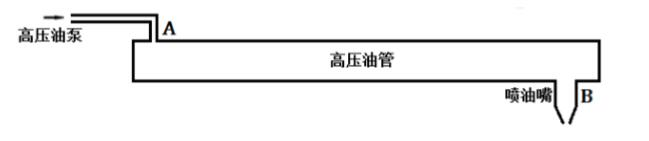
\includegraphics[width=1\textwidth]{youtube} %此时的图片宽度比例是相对于这个minipage的,不是全局
		\caption{高压油管示意图}
		\label{fig:youtube-picture}
	\end{minipage}
	\begin{minipage}[b]{0.4\textwidth} %所有minipage宽度之和要小于1,否则会自动变成竖排
		\centering %图片局部居中
		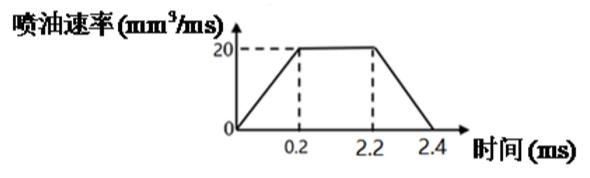
\includegraphics[width=1\textwidth]{penyousudu}%此时的图片宽度比例是相对于这个minipage的,不是全局
		\caption{喷油速率示意图}
		\label{fig:penyou-picture}
	\end{minipage}
\end{figure}
题目中某个高压油管的基本参数如下:

高压油管的内腔长度为 500mm,内直径为 10mm,供油入口
A 处小孔的直径为 1.4mm,通过单向阀开关控制供油时间的长短,单向阀每打开
一次后就要关闭 10ms。喷油器每秒工作 10 次,每次工作时喷油时间为 2.4ms,
喷油器工作时从喷油嘴 B 处向外喷油的速率如 \cref{fig:penyou-picture} 所示。高压油泵在入口 A 处提供的压力恒为 160 MPa,高压油管内的初始压力为 100 MPa。
\section{问题的提出}
\subsection{问题重述}
由题目给出的背景知识及三个问题可以分析出本文共需解决n个问题,通过解决这n个问题建立模型分析在高压油管中多个不同参数改变的情况下,如何调整油泵参数使发动机工作效率最大化。这些问题分别为:

\begin{enumerate}[label=\Roman*.]
	\item 要将高压油管内的压力尽可能稳定在 100 MPa 左右,如何设置单向阀每次开启的时长?\label{ques1} 
	\item 要将高压油管内的压力从 100 MPa 增加到 150 MPa,且分别经过约 2 s、5 s 和10 s 的调整过程后稳定在 150 MPa,单向阀开启的时长应如何调整? \label{ques2} 
	\begin{figure}[!h]
		\centering %图片全局居中
		%并排几个图,就要写几个minipage
		\begin{minipage}[b]{0.6\textwidth} %所有minipage宽度之和要小于1,否则会自动变成竖排
			\centering %图片局部居中
			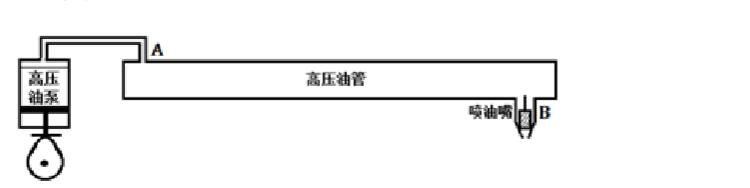
\includegraphics[width=1\textwidth]{realyoutube} %此时的图片宽度比例是相对于这个minipage的,不是全局
			\caption{高压油管实际工作示意图}
			\label{fig:realyoutube-picture}
		\end{minipage}
		\begin{minipage}[b]{0.39\textwidth} %所有minipage宽度之和要小于1,否则会自动变成竖排
			\centering %图片局部居中
			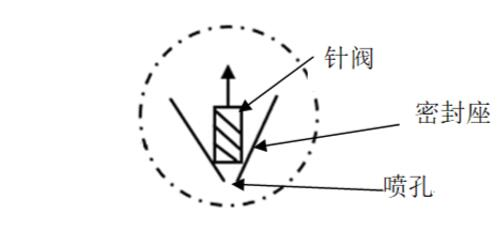
\includegraphics[width=1\textwidth]{muzzle}%此时的图片宽度比例是相对于这个minipage的,不是全局
			\caption{喷油器喷嘴示意图 }
			\label{fig:muzzle-picture}
		\end{minipage}
	\end{figure}
	\item 实际工作中,高压油管A处的燃油来自高压油泵的柱塞腔出口,喷油由喷油嘴的
	针阀控制。高压油泵柱塞的压油过程如\cref{fig:realyoutube-picture}所示,
	凸轮驱动柱塞上下运动。针阀的结构如\cref{fig:muzzle-picture}所示,
	燃油通过针阀的开闭喷出。在题目给出的基本参数条件下,
	确定凸轮的角速度,使得高压油管内的压力尽量稳定在100 MPa左右。\label{ques3} 
	
	\item 在上一问的基础上,再增加一个喷油嘴,每个喷嘴喷油规律相同,喷
	油和供油策略应如何调整?\label{ques4} 
	\begin{figure}[!h]
			\centering %图片局部居中
			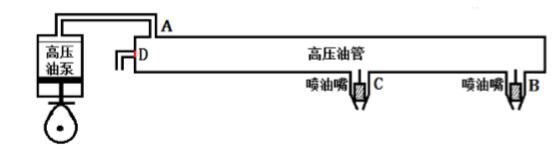
\includegraphics[width=0.8\textwidth]{doublemuzzle}
			\caption{具有减压阀和两个喷油嘴时高压油管示意图 }
			\label{fig:doublemuzzle-picture}
	\end{figure}

	\item 为了更有效地控制高压油管的压力,现计划在D处安
	装一个单向减压阀(\cref{fig:doublemuzzle-picture})。单向减压阀出口为直径为1.4mm的圆,打开后高压油
	管内的燃油可以在压力下回流到外部低压油路中,从而使得高压油管内燃油的压力减小。请给出高压油泵和减压阀的控制方案。 \label{ques5} 
\end{enumerate}
\subsection{问题分析}
\begin{enumerate}[label=\Roman*.]
	\item 根据题意,要尽可能维持高压油管内的压力为100Mpa,则单向阀门的入油质量和喷油嘴的出油质量应尽量维持在相等状态。由给出的公式可以求出不同压强条件下的燃油密度,再根据入油和出油的体积,建立方程式,解出维持100Mpa所需要的单向阀每次开启的时间。
	\item 如果要将燃油压强提升到150Mpa,其实质是高压油管中燃油质量的增加,先计算出燃油质量的增量,再建立相应方程式,解出单向阀每次开启的时间。其中,由于高压油管内的压强在时刻变化,需要做相应的近似处理。
	\item 首先根据附件1提供的数据,利用\textsc{Matlab}做出凸轮边缘曲线图像,分析可知,极径最大值与最小值的差即为柱塞运动到上、下止点的距离,记为$h$。根据克拉伯龙方程,以及附件1的数据可以近似求出凸轮在某一角度时,即可刚好打开单向阀门。 当凸轮继续运动到某一位置时,高压油泵内的压强下降到$100MPa$,单向阀门关闭。在这个过程中,一定质量的燃油被压进高压油管。
	喷油嘴通过针阀来控制喷油速率,其原理是当针阀升程为正时,假定针阀处于喷油嘴中心,此时针阀底端与密封座相应截面形成一个圆环:如果该圆环面积小于喷孔面积,则喷油速率取决于圆环面积大小;如果圆环面积大于喷孔面积,此时无论针阀的升程能否继续增大,喷油速率只取决于喷孔面积大小。通过以上分析,及附件2,拟合出每个周期内喷油速率随时间变化的函数及图像。即可计算出一个周期内喷孔喷孔喷出的燃油质量。维持100MPa压强的问题同样转化为问题\ref{ques1}中的进、出高压油管的燃油质量相等问题,可以建立方程,从而求解。
	\item
	\item
\end{enumerate}
\section{模型基本假设}
\begin{enumerate}
	\item 该品种燃油在题目中的温度和压强下不会被压燃
	\item 假设该油管的形状体积严格符合数据,没有误差
	\item 忽略外部因素对油管的影响并排除油管的机械故障
	\item 模型一的背景下高压油泵的出口压强保持恒定
	\item 模型一的特例中油管内的轻微压强变化可忽略
	\item
	\item
	\item
\end{enumerate}
\section{符号说明}
\begin{center}
	\begin{tabular}{cc}
		\toprule
		\makebox[0.3\textwidth][c]{符号}	&  \makebox[0.4\textwidth][c]{意义} \\ \midrule
		$V_{0}$	  & 高压油管容积($mm_{3}$)\\ 
		$K$       & 在$160MPa$下$\frac{E}{\rho}$的值\\
		$C$       & 流量系数\\
		$A$       & 高压油泵出油口面积($mm^{3}$)\\
		$A_{\text{孔}}$       & 喷油嘴喷孔面积($mm^{3}$)\\
		$A_{t}$       & t时刻喷油嘴实际喷油面积($mm^{3}$)\\
		$Q_{0}$   & 高压油管维持$100MPa$燃油流入油管速率($mm^{3}/ms$)\\
		$Q_{1}$   & 高压油管维持$150MPa$燃油流入油管速率($mm^{3}/ms$)\\
		$Q_{t}$   & t秒达到$150MPa$时燃油流入油管速率($mm^{3}/ms$)\\
		$\overline{Q}$    & 等效流入速率($mm^{3}/ms$)\\
		$Q_{c}$   & 单位周期内喷嘴喷油量($mm^{3}/100ms$)\\
		$t_{x}$   & 每次单向阀开启的时间($ms$)\\
		$t_{0}$   & 高压油管达到目标压强所需时间($ms$)\\
		$P_{0}$   & 初始时刻高压油管燃油压强($MPs$)\\
		$P_{t}$   & t时刻高压油管内的燃油压强($MPs$)\\
		$\rho_{0}$   & 初始时刻高压油管燃油压强对应的密度($mg/mm^{3}$)\\
		$\rho_{xMPs}$   & $xMPs$压强下燃油的密度($mg/mm^{3}$)\\
		$\overline{\rho_{c}}$   & 等效流出密度($mg/mm^{3}$)\\
		${\triangle M}$   & 始末时刻高压油管内部燃油质量差($mg$)\\
		\bottomrule
	\end{tabular}
\end{center}
\section{模型的构建与求解}
\subsection{维持油管恒压的单向阀开启时间模型}
根据题意,油泵的压强是理想情况下可以维持恒定的,只需要考虑出油和进油对高压油管部分的压强影响。因为压强这个数值不好处理,我们需要把这个物理量处理为质量。根据公式$\frac{E}{\rho} = \frac{\triangle P}{\triangle \rho}$可以得知油管内燃油密度和压强的联系,从而计算出$160MPa$下的密度。
\subsubsection{模型特例:高压油管内压强始终保持恒定}\label{case0}
在第一个小问题的假设下,可以把高压油管内部的燃油密度近似为定值。维持压强的问题就可以等价于进油口进油速率等于出油口出油速率。据此,可以得到以下方程
\begin{equation}
	\frac{ \rho_{160MPa}\times Q_{0}\times t_{x}}{t_{x}+10}=\frac{ \rho_{100MPa}\times Q_{c}}{100}\label{eq:ques1}
\end{equation}

其中,方程中的一些重要物理量 \footnote{如$Q_{c}$ , $t_{x}$,$A$等可以由题面数据直接得到或通过简单计算式得到的中间变量在此不列出} 由以下计算式解出:
\begin{equation*}
Q_{0} = C\times A\times \sqrt{\frac{2\times (160-100)}{\rho_{160MPa}}}\label{eq:ques1-1}
\end{equation*}

%对公式$\frac{E}{\rho} = \frac{\triangle P}{\triangle \rho}$移项积分可以得到
\begin{equation*}
	\int_{}^{}{\text{d}P} = \int_{}^{} \frac{E}{\rho}{\text{d}\rho}\label{eq:ques1-2}
\end{equation*}

代入$100MPa$时的数据可以得到,
\begin{equation}
P_{t} = E\ln\rho+452.9\label{eq:ques1-3}
\end{equation}



解出方程\cref{eq:ques1}得到时间$t_{x} = 0.2747ms$,该解即为问题\ref{ques1}的答案

\subsubsection{推广模型:压强发生改变后维持最终压强的单向阀开启时间模型}
高压油管压强在输油过程中发生改变会导致高压油泵的输入速率和喷嘴的输出密度变化,因此不再适用于特例情况下的单向阀开启时间模型。随着高压油管内压强的变大,输入速率逐渐变小而输出的密度在不断增大,``压强-时间''函数在达到稳定状态前可近似拟合 为一个$\ln x$型的函数\footnote{该结果根据附件3中的数据近似拟合得到},即以下形式:
\begin{equation}
	P_{t} = 100+\lambda\ln (t+1)\label{eq:ques2}	
\end{equation}

其中$t$为达到稳定前的自变量时间,$\lambda$为$t_{0}$时间到达稳定状态所对应的一个常数。在题面给出$t_{0}=2000ms$,$t_{0}=5000ms$,$t_{0}=10000s$的情况下,可以计算出他们相对应的$\lambda$值,然后利用\textsc{Matlab}绘制了下图,可近似看作高压油管内气体压强随时间变化的曲线。

\begin{figure}[!h]
	\centering 
	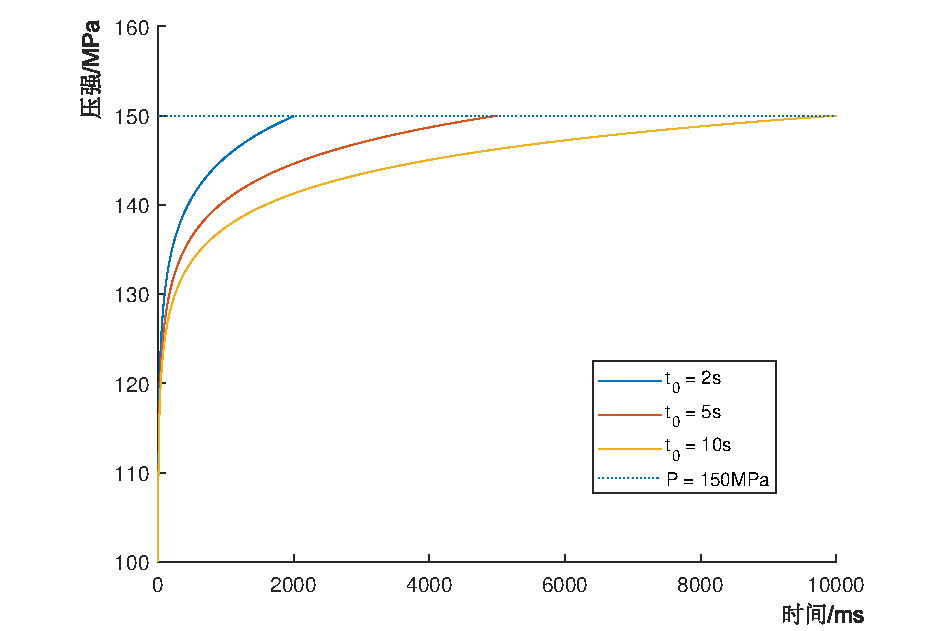
\includegraphics[width=0.8\textwidth]{P-tfigure}
	\caption{高压油管内气体压强随时间变化曲线}
	\label{fig:f(t)-picture}
\end{figure}
\newpage
首先,末态和初态的压强差,可以转化为质量的增加,那么高压油管内的压强从${100MPs}$增加为${150MPs}$,实质上是高压油管内燃油的质量增加${\triangle M}$,根据质量与密度和体积的关系,很容易计算出增量${\triangle M}$。
由于高压油管内的压强变化快,难以用模拟函数某一点的值近似表示该时刻的管内油压。所以用积分的平均值,来表示流入、流出油管的有效平均值,将变化的流入速率和变化的流出燃油密度,用其对应的有效平均值来近似等效。此时高压油泵的输入速率和喷嘴的输出密度都为恒定值,在$t_{0}$时间内,可以用$t$表示随着时间高压油管内燃油质量的增量,如果可以解出某个$t_{x}$值可以使其增量为${\triangle M}$,那么这个值即为所求单向阀开启时间。
\subsubsection{多种情况下该模型的求解}
根据上述对模型的描述,我们可以将模型抽象为以下三个等式:
\begin{enumerate}
	\item 等效平均流入速度的等式
	\begin{equation*}
	\overline{Q} = \frac{1}{t_{0}}\times \int_{0}^{t_{0}} C\times A\times \sqrt{\frac{2\times (160-P_{t})}{P_{160MPa}}}{\text{d}t}\label{eq:ques2-1}	
	\end{equation*}
	\item 等效平均流出密度的等式\footnote{该等式中的常数由计算式\cref{eq:ques1-3}得到}
	\begin{equation*}
	\overline{\rho_{c}} = \frac{1}{t_{0}}\times \int_{0}^{t_{0}} e^{\frac{P_{t}-452.9}{E}}{\text{d}t}\label{eq:ques2-2}	
	\end{equation*}
	\item 该模型的求解方程
	\begin{equation}
	t_{0}\times(\frac{\overline{Q}\times t_{x}}{t_{x}+10}\times \rho_{160MPa}-\frac{Q_{c}}{100}\times \overline{\rho_{c}})-\triangle M = 0\label{eq:ques2-3}	
	\end{equation}
	使用\textsc{Matlab}解出方程\cref{eq:ques2-3},所得到的解即是我们所需要求的阀门开启时间。以下分别就$t_{0}$的几种取值讨论解的结果。
\end{enumerate}
\paragraph{$t_{0}=2000ms$时}~{}

代入函数\cref{eq:ques2}可计算出$\lambda=6.57$,运用该值解方程\cref{eq:ques2-3},解得$t_{x} =2.7511$显然不符合事实。可推断在$2000ms$内无法将高压油管内燃油的压强提升至$150MPa$。为了验证这一论断,我们不妨做一个极限的假设:假设在这$2000ms$内更多的燃油并不会使高压油管内压强增大,即高压油泵能在$2000ms$内一直以最大的速率向油管输入燃油,在到达$2000ms$时燃油压强也无法到达$150MPs$。显然在该条件下没有解。

\paragraph{$t_{0}=5000ms$时}~{}

代入函数\cref{eq:ques2}可计算出$\lambda=5.87$,运用该值解方程\cref{eq:ques2-3},解得$t_{x} = 1.5160ms$。该值即为调整时间内单次开启单向阀的时长。
\paragraph{$t_{0}=10000ms$时}~{}

代入函数\cref{eq:ques2}可计算出$\lambda=5.43$,运用该值解方程\cref{eq:ques2-3},解得$t_{x} = 1.1524ms$。该值即为调整时间内单次开启单向阀的时长。

\paragraph{压强达到$150MPa$时}~{}

当压强稳定在$150MPa$时,该模型又回到了特例的条件下,运用\ref{case0}的结论可以得到$t_{x} = 0.7383ms$。该值即为稳定后没次单向阀的开启时间

\subsubsection{结果分析}

综上,可以得到问题\ref{ques2}的结果
\begin{enumerate}
	\item $t_{0}=2000ms$时,因时长太短,无法通过开启单向阀使高压油管内压强上升到指定值。
	\item $t_{0}=5000ms$时,应调整单项阀的开启时长为稳定前每次开启$6.7607ms$,稳定后每次开启$1.3794ms$。
	\item$t_{0}=10000ms$时,应调整单项阀的开启时长为稳定前每次开启$2.7771ms$,稳定后每次开启$1.3794ms$。
\end{enumerate}
\subsection{维持高压油管压强的凸轮角速度模型}

\section{总结}
\subsection{模型的评价}
\subsubsection{模型的优点}
\subsubsection{模型的缺点}
\subsection{模型的改进}
\subsection{模型的推广}

%参考文献
\begin{thebibliography}{9}%宽度9
	\bibitem{bib:one}
\end{thebibliography}
\newpage
\begin{appendices}
\section{计算单项阀开启时间的\textsc{Matlab}代码}
\begin{tcode}
%高压油管的容积为V_0
%一次周期的喷油量记Q_c
%100MPa压强下,燃油的密度记为R_0
%160MPa压强下,燃油的密度记为R_1
%150MPa压强下,燃油的密度记为R_2
%设维持100MPa单向阀门开启一次时常为t_0;
V_0 = pi*5^2*500;
R_0 = 0.850;
syms R
R_1 = fzero(@(R) 2786.4*log(R)+452.9-160,1);
R_2 = fzero(@(R) 2664.3*log(R)+452.9-150,1);
%syms P
%equ = (0.0289*P^2+3.0765*P+1571.6)*log(R) + 459.2 - P == 0;
%R_P = solve(equ,R,'ReturnConditions',true);
C = 0.85;
r = 0.71;
A = pi*r^2;
Q_0 = C*A*(2*(160-100)/R_1)^0.5;
Q_c = 20*(2+2.4)/2;
syms t_0
fun_0 = @(t_0) (R_1*Q_0*t_0/(t_0+10)-R_0*Q_c/100);
t_0 = fzero(fun_0,0.5);
%设提升至150MPa 单向阀门开启一次时长为t_1,t_2,t_3
%分别对应经过2s 5s  10s的调整后稳定
%设油管内燃油的质量差为deltaM mg
deltaM = (R_2 - R_0)*V_0;
%设在t_1、t_2、t_3情况下,等效进油量分别为Q_1 Q_2 Q_3
syms t
%计算t_1
Q_1 = integral(@(t) C*A*(2*(60-6.57*log(t+1)/R_1)).^0.5,0,2000)/2000;
R_c1 = 0.88;
fun_1 = @(x) 2000*(Q_1*x/(x+10)*R_1-Q_c/100*R_c1) - deltaM;
t_1 = fzero(fun_1,10);
test1 = fun_1(2000);
%在假设的模拟之下,每次开启阀门的时间为2.7511ms

%计算t_2
Q_2 = integral(@(t) C*A*(2*(60-5.87*log(t+1)/R_1)).^0.5,0,5000)/5000;
R_c2 = 0.88;
fun_2 = @(x) 5000*(Q_2*x/(x+10)*R_1-Q_c/100*R_c2) - deltaM;
t_2 = fzero(fun_2,5);
test2 = fun_2(5000);
%在假设的模拟之下,每次开启阀门的时间为1.5160ms

%计算t_3
Q_3 = integral(@(t) C*A*(2*(60-5.43*log(t+1)/R_1)).^0.5,0,10000)/10000;
R_c3 = 0.88;
fun_3 = @(x) 10000*(Q_3*x/(x+10)*R_1-Q_c/100*R_c3) - deltaM;
t_3 = fzero(fun_3,0.5);
%在假设的模拟之下,每次开启阀门的时间为1.1524ms


%维持150MPa所需的开启时长
Q_00 = C*A*(2*(160-150)/R_1)^0.5;
syms t_4
fun_4 = @(t_4) (R_1*Q_00*t_4/(t_4+10)-R_2*Q_c/100);
t_4 = fzero(fun_4,0.5);
%维持150MPa每次开启时间为0.7383ms
\end{tcode}
\end{appendices}


\end{document}
